\documentclass[10pt,a4paper]{revtex4-2}
\usepackage[a4paper, margin=1in]{geometry}
\usepackage[utf8]{inputenc}
\usepackage{amsmath}
\usepackage{amsfonts}
\usepackage{amssymb}
\usepackage{graphicx}   


\newcommand{\sign}{\text{sgn}}
%\newcommand{\avgk}[1]{<#1>_i}
\newcommand{\avgk}[1]{\overline{#1}_i}

\usepackage{lineno} 



\begin{document}

\linenumbers % Activate line numbering

\title{Analytical Bayesian Inference of Yeast
DNA Replication Reveals Intrinsic Origin Strengths and Activation Delays}
\author{Dario D'Asaro}
\email{correspondence: dario.dasaro@ens-lyon.fr}
\affiliation{%
 Laboratoire de Biologie et Modélisation de la Cellule, École Normale Supérieure de Lyon, CNRS, UMR5239, Inserm U1293, Université Claude Bernard Lyon 1, 46 Allée d’Italie, 69007 Lyon, France
}%
\affiliation{%
 École Normale Supérieure de Lyon, CNRS, Laboratoire de Physique, 46 Allée d’Italie, 69007 Lyon, France
}%

\author{Diletta Ciardo}
\email{correspondence: diletta.ciardo@bio.ens.psl.eu}
\affiliation{IBENS} 

\author{Arach Goldar}
\email{correspondence: Arach.goldar@cea.fr }
\affiliation{CEA} 


\author{Olivier Hyrien}
\email{correspondence: olivier.hyrien@bio.ens.psl.eu}
\affiliation{IBENS} 

\author{Laurent Lacroix}
\email{correspondence: laurent.lacroix@bio.ens.psl.eu}
\affiliation{IBENS} 

\author{Beno\^it Le Tallec}
\email{correspondence: letallec@bio.ens.psl.eu}
\affiliation{IBENS} 

\author{Benjamin Audit}
\email{correspondence: benjamin.audit@ens-lyon.fr}
\affiliation{%
 École Normale Supérieure de Lyon, CNRS, Laboratoire de Physique, 46 Allée d’Italie, 69007 Lyon, France
}%


\author{Daniel Jost}
%\email{correspondence: dario.dasaro@ens-lyon.fr}
\affiliation{%
 Laboratoire de Biologie et Modélisation de la Cellule, École Normale Supérieure de Lyon, CNRS, UMR5239, Inserm U1293, Université Claude Bernard Lyon 1, 46 Allée d’Italie, 69007 Lyon, France
}%
\affiliation{%
 École Normale Supérieure de Lyon, CNRS, Laboratoire de Physique, 46 Allée d’Italie, 69007 Lyon, France
}%


\author{Jean-Michel Arbona}
\email{correspondence: jeanmichel.arbona@univ-amu.fr}
\affiliation{Aix Marseille University, CNRS, IBDM, Turing Centre for Living Systems, Parc Scientifique de Luminy, 13288 Marseille, France}

\maketitle


\section{Abstract}
We present an analytical framework for modeling eukaryotic DNA replication, enabling Bayesian inference of origin number, their intrinsic 
strengths (\(\lambda\)) and activation delays from experimental Replication Fork Directionality (RFD) data. 
By deriving closed-form expressions for RFD and Mean replication Timing under exponential and Weibull
 firing-time distributions, we eliminate the need for stochastic simulations, 
  achieving 0.95–0.98 correlation with yeast RFD profiles. 
  Our bayesian method resolves ~650 origins in \textit{S. cerevisiae}. 
  We demonstrate that RFD discontinuities encode observed efficiencies (\(E\)), 
  the passivation-adjusted probability of origin firing. Critically, 
  the RFD depends on both \(\lambda\) and fork speed (\(v\)), 
  such that \(\lambda\) can be inferred from RFD when \(v\) is known (e.g., via experimental measurements). 
  We demonstrate a simple relationship that explain how the neighborhood of an origin modulates its intrinsic efficiencies and
  give rise to the observed efficiency. 
  Our framework identifies about 50 origins with biologically significant delays (\(\geq 1\) minute), revealing regulated 
  activation kinetics undetectable by existing methods. By quantifying how \(\lambda\) and delays shape replication timing landscapes,
  this work confirm yeast as a paradigm organism for studying DNA replication control mechanisms.
%\section{Target journal}
%Bayesian inference of origin firing time distributions, origin interference and licencing probabilities from Next Generation Sequencing data (NAR)
%
%Mathematical modeling of genome replication (Phys Rev E)
%
%Genome research


\section{Introduction}

\paragraph*{Challenges of Eukaryotic DNA Replication}
DNA replication is a fundamental process ensuring genomic stability during cell division. 
In eukaryotes, replication initiates at hundreds to thousands of origins distributed across chromosomes \cite{DePamphilis2010},
with their timing and efficiency tightly regulated. 
Two main categories of experimental approaches provide complementary perspectives on replication.
The first comprises ChIP-seq assays that measure the chromatin binding of replication initiation complexes, 
such as the Origin Recognition Complex (ORC) and the Minichromosome Maintenance (MCM) helicase \cite{Dellino2013,Kirstein2021,Miotto2016,Foss2021,Li2023}. 
These factors are essential for origin licensing in G1 phase, and their genomic occupancy serves as an 
experimental proxy for an origin’s intrinsic firing potential \cite{Dellino2013}. 
Importantly, intrinsic strength is not determined solely by factor binding: it can be modulated by chromatin regulators such as Sir2, 
which alter the local protein state and thereby affect licensing efficiency \cite{Hayashi2009,Hoggard2020}. 
Thus, ChIP-seq reflects the potential for origin activity, while additional regulatory mechanisms fine-tune how this potential is realized in vivo.

It is also critical to distinguish between the \textit{licensing} of replication origins and their \textit{control during S-phase}. 
Licensing occurs in G1, when ORC, Cdc6, and Cdt1 load the MCM helicase onto DNA, thereby establishing the pool of potential origins. 
This step defines whether an origin is competent to fire but does not guarantee activation. 
During S-phase, licensed origins compete for limiting firing factors and may be silenced by incoming replication forks through the passivation mechanism. 
For example, even two intrinsically strong origins can interfere: if one origin fires first, the advancing fork can replicate and thereby passivate its neighbor before activation occurs. 
This phenomenon gives rise to the concept of observed efficiencies (\(E\)), 
the passivation-adjusted probability of origin firing. 
The central modeling challenge is thus to connect intrinsic origin properties, regulatory mechanisms, 
and population-level passivation-adjusted quantities observables such as mean replication timing (MRT) \cite{Long2020,Hansen2010,Zhao2020} and 
replication fork directionality profiles \cite{Petryk2016,Wu2018}.

\paragraph*{Advances in Experimental Techniques}
Recent experimental breakthroughs, such as OK-Seq \cite{Petryk2016} and FORK-Seq \cite{Hennion2020}, 
have enabled genome-wide mapping of Replication Fork Directionality (RFD) \cite{Wang2021}, 
initiation density, and fork speeds \cite{Theulot2022} in asynchronous cell populations. 
These methods bypass synchronization-induced perturbations, offering unprecedented insights. 
Single-molecule studies by Gauthier et al. \cite{Gauthier2012} further demonstrated how local origin firing patterns influence replication dynamics. 
Despite these advances, computational methods to infer intrinsic origin strengths along the genome (\(\lambda\),
defined as the inherent firing rate per unit time) remain limited.

\paragraph*{Limitations of Existing Computational Approaches}
Previous methods face significant challenges. 
For example, Bazarova et al. \cite{Bazarova2019} used stochastic simulations based on Retkute et al.’s model \cite{Retkute2012} to estimate origin efficiencies 
from RFD data. However, their reliance on simulating thousands of cells restricted analyses to small systems
of three origins at a time, neglecting interdependencies between neighboring origins. 
Similarly, Arbona et al. \cite{Arbona2023} combined neural networks with replication timing data but 
required computationally intensive iterative training. Bayesian methods \cite{Bazarova2019} have also 
shown that reduced licensing probabilities and origin passivation contribute to replication control, 
yet these approaches remain constrained by computational bottlenecks.

A recent study by Berners-Lee et al. \cite{BernersLee2025} 
advanced the field by developing a stochastic, whole-genome model of 
\textit{S.~cerevisiae} replication timing in which origins compete for a limited pool of firing factors. 
At kilobase resolution, their model successfully reproduced mean replication timing, inter-origin distances, 
origin efficiencies, and replication fork directionality. 
This work strongly supports the view that competition among origins, together with limiting firing factors, 
is a major determinant of replication timing. 
Nevertheless, the model relies on extensive stochastic simulations, 
limiting its ability to provide closed-form links between intrinsic strength, observed efficiency, 
and experimental readouts such as MRT and RFD.

\paragraph*{Our Contributions}
Here, we address these limitations by developing a novel analytical 
framework that provides closed-form solutions for RFD and Mean Replication Timing (MRT) 
under both exponential and more biologically realistic Weibull firing-time distributions.
This approach eliminates the computational expense of stochastic simulations, 
enabling rapid, genome-wide Bayesian inference of intrinsic origin strengths ($\lambda$) 
and activation delays. 
Our model yields critical mechanistic insights, demonstrating that 
RFD discontinuities directly encode the observed, passivation-adjusted firing efficiency ($E$).
We establish the theoretical relationship between RFD, $\lambda$, and fork speed ($v$), 
allowing for the inference of absolute origin strengths when fork speed is known. 
Furthermore, under an exponential firing model, we derive the simple but powerful relationship 
$E_i = \lambda_i \cdot \text{MRT}(x_i)$, which analytically clarifies the often-conflated distinction
between intrinsic strength and observed efficiency. 
Applying this scalable framework to \textit{S. cerevisiae},
we resolve approximately 650 origins and identify about 50 with biologically significant activation
delays ($\geq 1$ minute), revealing a layer of regulated activation kinetics previously undetectable
by other methods.

\paragraph*{Significance}
Our work bridges the gap between theoretical models and data-driven analysis, 
offering a robust tool to study replication dynamics under diverse conditions. 
By distinguishing \textbf{intrinsic origin strengths (\(\lambda\))} from \textbf{observed efficiencies (\(E\))},
with a simple relation-ship, we clarify a critical distinction. 
We validate our framework on synthetic data and apply it to experimental yeast datasets,
revealing biologically significant delays in about 50 origins. 
This framework establishes yeast as a paradigm system for dissecting DNA replication control mechanisms.
Studies of genetic variation in replication timing underscore the importance of such mechanistic models
for understanding genomic stability \cite{Koren2014}.

\section{Model}

In Retkute et al. \cite{Retkute2012}, replication is modeled by a set of discrete origins localised on a chromosome. 
The probability for an origin $i$ to be activated is $p_i(t) =q_i p(t) $ with $p(t)$ any probability distribution and $q_i$ the efficiency of licensing of one origin. In the following sections we set the licensing probability to 1, but we will come back on this hypothesis at the end of the modeling section.  An origin can still be not activated because of the passivation by neighbor origins.
$p(t)$ in a first time represents an arbitrary probability distribution of firing, but later on will be fixed to be exponential or Weibull with parameter $k=2$. If $t<0$ then $p(t)=0$. The probability for a fork starting from origin $i$ located at position $x_i$ to reach the point $x$ at $t$ is:

\begin{equation}
p_i(x,t) =  p \left(t-\frac{|x-x_i|}{v}\right) 
\end{equation} 
which is a delay of the initial probability distribution due to the propagation of the fork. 

The probability that another fork $j$ arrives at $x$ later than $t$  is given by

\begin{equation}
M_j(x,t) = \int_t^{\infty} p_j(x,\tau) d\tau
\end{equation} 


Starting from these equations it can be shown Sec. \ref{seq:MRT} that:

\begin{equation}\label{mrt0s}
MRT(x) =  \int_{0}^{\infty} \prod_{i} M_i(x,t) dt
\end{equation}

which is considerably simplified with respect to the original formulation of Retkute et al. \cite{Retkute2012} which combines both 
Eq. \eqref{omrt} and Eq. \eqref{op}. This allows the analytical derivation of MRT and $RFD=v\frac{dMRT(x)}{dx}$ and $E_i$ , the observed efficiency of the origin $i$ for two types of distribution of origin firing.

We first evaluate these quantities for the exponential distribution, followed by the Weibull case with shape parameter k=2. These two probability distributions are plotted 
in Fig \ref{fig:valmodel} A,E respectively.





\subsection{Exponential Firing Distribution}
The replication dynamics for a system of \(N\) origins with exponentially distributed firing times (\(p_i(t) = H(t)\lambda_i e^{-\lambda_i t}\) for origin $i$), with H(t) the Heaviside function, yields closed-form solutions for MRT and RFD. 

We define \(t_i = \frac{|x - x_i|}{v} + t_i^S\) at $x$, as the total delay for a fork from an origin at \(x_i\) to reach position \(x\). This delay comprises two components: the propagation time \(\frac{|x - x_i|}{v}\) (time for the fork to travel the distance \(|x - x_i|\) at speed \(v\)) and an optional activation delay \(t_i^S\) (mimicking regulatory delays in origin firing).

To compute \(\text{MRT}(x)\), we first sort the \(n\) origins by their arrival times \(t_i\) (ascending order). The integration is partitioned into intervals where only subsets of origins contribute. Between \(t \in [0, t_1)\), all \(M_i(t,x) = 1\) (no forks have arrived), while for \(t \in [t_i, t_{i+1})\), only the first \(i\) origins contribute non-trivially.

After calculation (App. \ref{appendix:exponential}), the MRT at position \(x\) is:
\begin{equation}\label{eq:mrt_exp}
\text{MRT}(x) = t_1 + \sum_{i=1}^{n}\frac{1}{\sum_{j=1}^i \lambda_j}\left[e^{-\sum_{j=1}^i \lambda_j(t_i - t_j)} - e^{-\sum_{j=1}^i \lambda_j(t_{i+1} - t_j)}\right].
\end{equation}
Similarly it is possible to compute the variance of the MRT (Sec. \ref{appendix:exponential}) which can be discriminative for the underlying activation process.

\paragraph{RFD Derivation:}
The RFD is derived as the spatial derivative of MRT scaled by fork speed:
\begin{equation}\label{eq:rfd_exp}
\text{RFD}(x) = v \frac{d}{dx}\text{MRT}(x),
\end{equation}
where differentiation accounts for the linear dependence \(t_i = \frac{|x - x_i|}{v} + t_i^S\) (see App. \ref{appendix:exponential} for details).

\paragraph{Observed Efficiency (\(E_i\)):} 
The observed efficiency or the passivation-adjusted firing probability is defined as:
$E_i = \int_0^{\infty} p_i(x_i,t)\prod_{j \neq i} M_j(x_i,t)dt$ which corresponds to the probability that 
the fork $i$ is activated multiplied by the probabilities that other forks arrive later,
and this intergrated over the whole S-phase.
The exponential model yields (Sec. \ref{appendix:exponential}):

\begin{equation}\label{eq:ei_exp}
E_i = \lambda_i \cdot \text{MRT}(x_i) \quad \text{(Observed efficiency vs. intrinsic strength relationship)}
\end{equation} 
 valid when \(t_i^S = 0\). Delays \(t_i^S \neq 0\) invalidate this relationship if forks preempt origin activation (Sec. \ref{appendix:exponential}).

\subsection{Weibull Firing Distribution (shape parameter \(k=2\))}
For gradual origin activation, the Weibull distribution (\(k=2\)) with \(p(t) = 2tH(t)\lambda_i^2e^{-(\lambda_i t)^2}\) provides a more realistic model. The Weibull model reduces to the exponential case when \(k=1\). The MRT becomes:
\begin{equation}\label{eq:mrt_weibull}
\text{MRT}(x) = t_1 + \sum_{i=1}^{n} \text{MRT}_i(x),
\end{equation}
where each term \(\text{MRT}_i(x)\) involves Gaussian integrals:
\begin{equation}
\text{MRT}_i(x) = \frac{1}{\sqrt{\avgk{1}}} e^{\avgk{t}^2/\avgk{1} - \avgk{t^2}} \int_{\sqrt{\avgk{1}}(t_i - \avgk{t}/\avgk{1})}^{\sqrt{\avgk{1}}(t_{i+1} - \avgk{t}/\avgk{1})} e^{-u^2} du,
\end{equation}
with \(\avgk{t} = \sum_{j=1}^{i} \lambda_j^2 t_j\) and \(\avgk{1} = \sum_{j=1}^{i} \lambda_j^2\). While these integrals involve the error function (\(\text{erf}\)), they are computationally efficient
in practice: standardized approximations for \(\text{erf}\) are implemented in 
numerical libraries, eliminating the need for explicit numerical integration during evaluation.

The RFD derivation parallels the exponential case but requires differentiating error function terms. (Sec. \ref{appendix:weibull}).

\begin{figure}[ht]
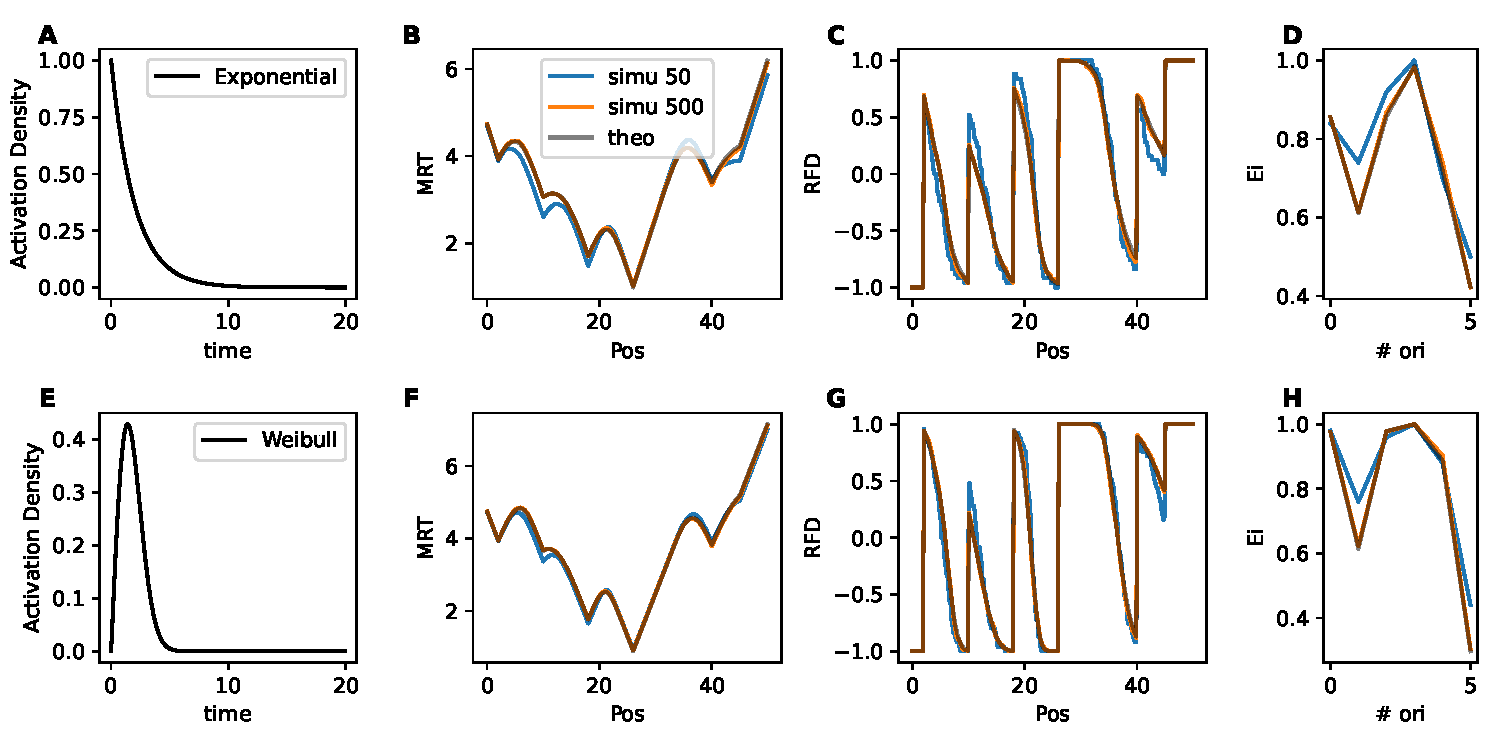
\includegraphics[width=1.\textwidth]{figures/theo.pdf}
\caption{
Analytical vs. simulated profiles for exponential (A--D) and Weibull \(k=2\) (E--H) models. 
\textbf{(A/E)} Activation function for $\lambda=2$,\textbf{(B/F)} MRT, \textbf{(C/G)} RFD, and \textbf{(D/H)} observed efficiencies \(E_i\) show near-perfect agreement. 
Simulations involve stochastic firing time sampling and fork propagation at constant speed, with origins passivated (silenced) 
if preempted by neighboring forks. For both models, 50 simulations (blue lines) exhibit residual noise, while 500 simulations (red lines)
 converge to the analytical solution (black lines). 
}\label{fig:valmodel}
\end{figure}

For computing any quantity at a given point x, it amounts in practice to compute $t_i$ from each origin and then computing the various sums. In Fig \ref{fig:valmodel} we compare Monte Carlo simulation with N=50/N=500 replicates to the analytical formula. We choose parameters by hand to have combination of origin strength and delay (SI ).
For the simulation, the activation time of an origin is drawn  according to its corresponding activation law, and if an activation time is higher that the time it takes for another origin to reach the position of the first mentioned origin, this origin is passivated. We can observe that a simulation with 500 replicates perfectly overlaps with the analytical formula. The difference between the two firing models are small but can be observed as a smoother MRT and RFD profile for the Weibull distribution.  


\subsection{Including partial licensing of origins}

One hypothesis of the model is that all origins succeed in licensing. From experimental evidence it is not clear that it is the case. This hypothesis was used to simplify the analytical framework. Two main questions then arise: i) is it possible to include it in the analytical framework? ii) if this is present in the data, what is the impact of fitting with a model that does not include it? 
It is possible to carry on the computation taking into account $q_i \neq 0$. The resulting MRT, is then a weighted sum of : the MRT where all the origins are taken into account, plus the MRT where one origin is excluded for all origins, plus the MRT where all possible couple of origins are excluded and so on:

\begin{equation}
MRTq(x,[q_1,..q_i,...q_n]) = w_{\varnothing} MRT(x,\varnothing) +  \sum_i w_{[i]} MRT(x,[i]) +  \sum_i\sum_j w_{[i,j]} MRT(x,[i,j]) + ...
\end{equation}
with $MRT(x,\varnothing)$, the classical MRT  where no origin has been excluded, $MRT(x,[i])$, the MRT where we discard origin $i$ from the set of origin, and so on.
The weights are: $w_{\varnothing} = \prod_j q_j$,  $w_{[i]} = \prod_{j\neq i} q_j (1-q_i) $.

The full MRT is thus a combinatorial sum of all possible combinations of active origin.
Computing it would result in a combinatorial computation and would result in being impractical. However if one make the hypothesis that most of the origin have a rather high probability to have licensing, it is possible to approximate the full MRT by
 adding perturbation due to one origin being not licensed for all origin in a reasonable amount of time:

\begin{equation}
MRT_{approx}(x,[q_1,..q_i,...q_n]) = \frac{w_{\varnothing}}{w_{\varnothing}+\sum_i w_{[i]}} MRT(x,\varnothing) +  \sum_i \frac{w_{[i]}}{w_{[0]}+\sum_i w_{[i]}} MRT(x,[i])
\end{equation}
In practice it could be be carried by computing $MRT(x,\varnothing)$ and only part of  $MRT(x,[i])$ where the origin i was active and should be removed from the computation, the other parts of the MRT being the same. In the following work we did not implement this correction. We will discuss the impact of this hypothesis on the discussion.


\section{Analysis of RFD}

\subsection{RFD information content: Inferring Absolute Origin Efficiencies from RFD Data}

Our analytical result allows us to reveal an interesting symmetry:
the RFD profiles in the exponential case is inherently invariant under simultaneous rescaling of 
fork speed (\(v \to fv\)) , intrinsic efficiencies (\(\lambda_i \to f\lambda_i\)) and
 delay (\(t_i^S \to t_i^S/f\)) for any \(f > 0\). 
 This symmetry arises because RFD formula contains terms such as\(t_i \lambda_j = \frac{|x_i - x_j|}{v} \cdot \lambda_j\) and 
ratio of $\lambda_i$ which remain unchanged under such transformations. 
Consequently, RFD alone cannot uniquely resolve both \(v\) , \(\lambda_i\) and $t_i^S$. 
However, if the fork speed \(v\) is independently determined (e.g., experimentally measured), 
this invariance is broken, and RFD encodes \textit{absolute} intrinsic efficiencies through 
the \textit{passivation mechanism}. 

Specifically, the RFD discontinuity (``jump") at an origin location \(x_i\) corresponds to twice its observed efficiency (Sec. \ref{seq:rfdj})
\begin{equation}
\text{RFD jump at } x_i \approx 2E_i,
\end{equation}
where \(E_i\) is the probability that origin \(i\) fires before being passivated. 
We illustrate how one can obtain intrinsic strength even wen using passivation adjusted quantities,
for a two-origin system with exponential firing dynamics. For the observed efficiency Eq. \ref{eq:ei_exp} becomes:
\begin{equation}
E_1 = 1 - e^{-\lambda_1 t_2} \left(1 - \frac{\lambda_1}{\lambda_1 + \lambda_2}\right),
\end{equation}
with \(t_2 = \frac{|x_2 - x_1|}{v}\). Here, the exponential term \(e^{-\lambda_1 t_2}\) introduces 
dependence on the absolute value of \(\lambda_1\), enabling calibration against the physical 
timescale \(t_2\) when \(v\) is fixed.

When origins are highly efficient (\(E_i \sim 1\)), the term \(e^{-\lambda_1 t_2}\) becomes negligible
 (\(\lambda_1 t_2 \to \infty\)), and the relationship between \(E_i\) and \(\lambda_i\) loses sensitivity.
  In this regime, absolute efficiencies cannot be reliably estimated from RFD alone.

\subsection{Estimating model parameters}


\subsubsection{Estimation and Model Selection}

To infer the model parameters (intrinsic strengths $\lambda_i$ and delays $t_i^S$) from experimental RFD data, we need a robust statistical method. A straightforward approach is to find the parameters that minimize the difference (e.g., mean squared error) between our model's predicted RFD profile and the experimental one. While fast, this method does not easily allow us to compare the performance of fundamentally different models, such as the Exponential versus the Weibull firing model.

To address this, we adopted a Bayesian framework. 
This approach not only estimates the most likely value for each parameter but also quantifies the 
uncertainty of that estimate. Crucially, it provides a formal way to compare different models. 
We explored several computational techniques to implement this, including Maximum a Posteriori (MAP) \cite{Bishop2006}, 
the Laplace approximation \cite{Bishop2006,MacKay2003}, and Automatic Differentiation Variational Inference (ADVI) \cite{Kucukelbir2017}.

These methods allow us to calculate the Evidence Lower Bound (ELBO), 
a score that reflects how well a given model explains the experimental data. 
The ELBO give a higher score to the model that perform the best compromise between fit and efficiency in terms of parameters.
It thus penalizes overfitting.
By comparing ELBO scores, we can select the best model (e.g., Weibull with delays) and the optimal number of origins.
While variational methods like ADVI and Laplace can slightly underestimate parameter uncertainty \cite{Blei2017}, 
they proved highly effective for model selection in our tests. 
We found that the Laplace method provided a good balance of speed and accuracy, making it ideal for our genome-wide analysis. 

Further details on the statistical implementation are provided in the Appendix (\ref{sup:detail}).

RFD computation requires accounting for origin interference within replication fork reach 
($\sim$50 kb at 2.5 kb/min \cite{Theulot2022}). 
We evaluated model performance as a function of neighborhood size (origins considered per locus). 
Beyond 5–6 origins, the correlations plateaued. 
As the method is efficient we choose to retain all origins, but a threshold on the distances could be included, for example in truncating the origins
further away than two lengths that one fork can travel during S-phase.
Notably while the RFD or MRT are computed at specific locus, the position of the origin can be chosen in a continuous manner and could even be optimized. However, here we did not optimize it.

The same origin detection pipeline was applied to synthetic and experimental RFD to select a given number of origins (Appendix~\ref{app:origin_detect}).

So the general full pipeline can be summarized as follow: 
given RFD data, select different sets of origins positioning based on a set of thresholds.
Then for each origins set of origin, performs Laplace method for the different Exponential and Weibull models 
with and without delay. 
Then select the model which is a couple of model choices and origin number. 
Then we can compute the average value and standard deviation of the parameters.



\subsubsection{Analysis of the performance on synthetic datasets}

\begin{figure}
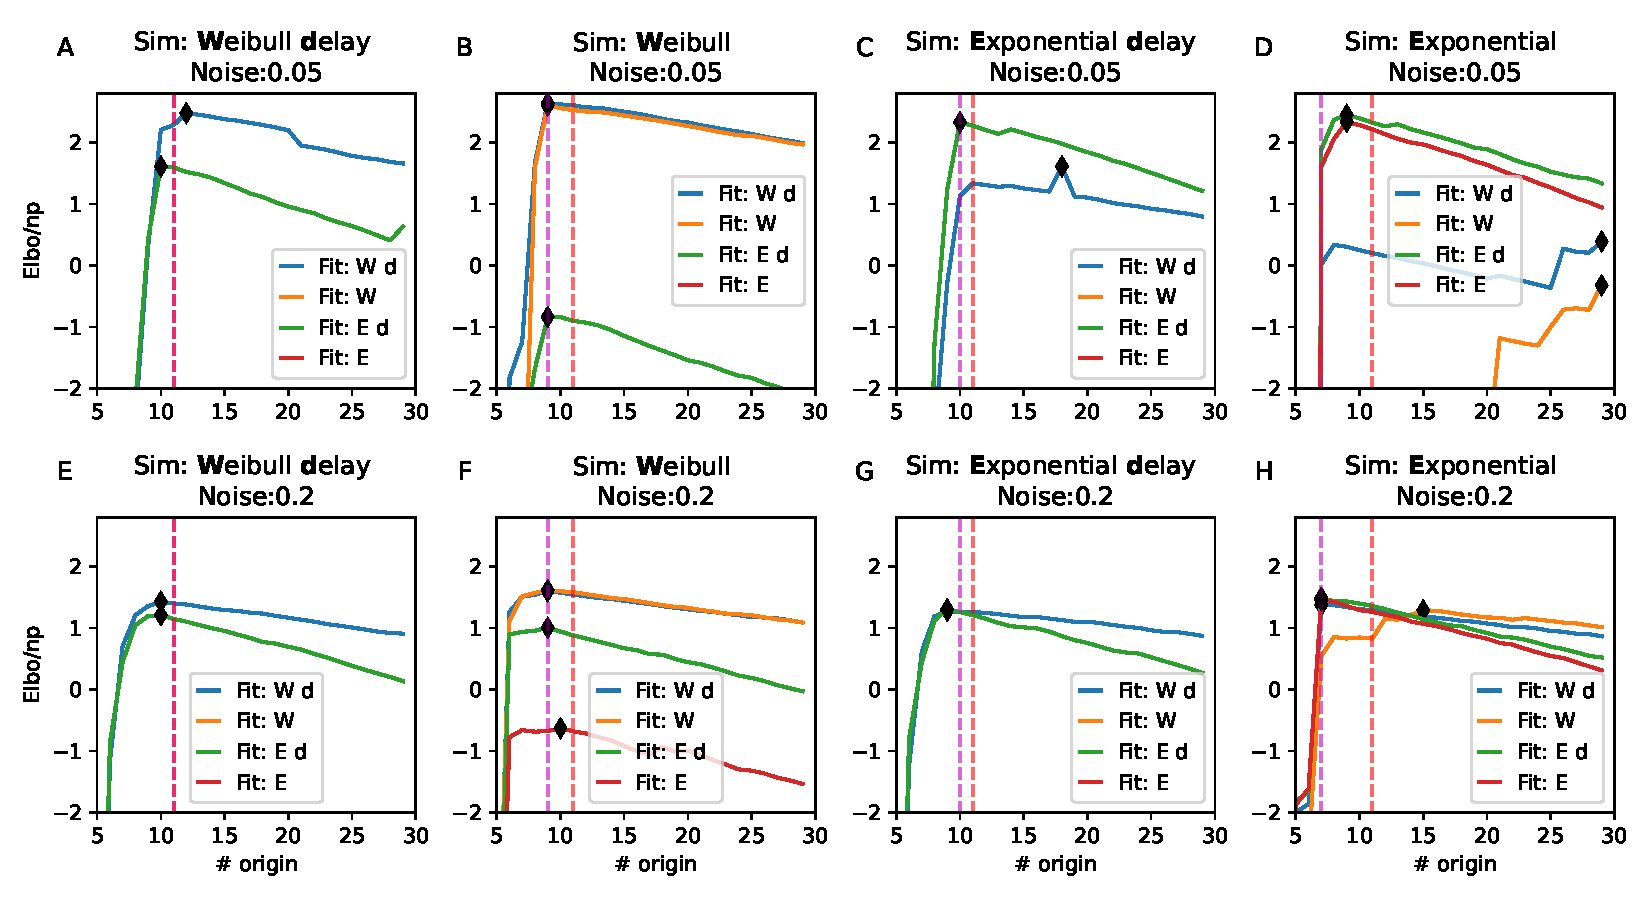
\includegraphics[width=1\textwidth]{figures/analyse-synthetic.pdf}
\caption{Evaluation of ELBO as a function of the number of origins under different noise levels and firing models.
The eight plots are grouped into two panels: A-D represent simulations with low noise 0.05 (in RFD unit), 
and E-H represent simulations with high noise (0.2). Each subfigure corresponds to data generated with simulation with specific firing model 
(Exponential or Weibull) with or without delay. The curves displayed corresponds to fit with the different models. They include: "Weibull with delay" (blue),
"Weibull" (orange), "Exponential with delay" (green), "Exponential" (red). The orange vertical dashed line indicate the total number of origin. 
The purple one the number of origin with observed efficiency higher than 0.05}\label{fig:synthetic}
\end{figure}

We evaluated the model selection procedure by simulating data using one model and computing the ELBO for four models: Exponential with or without time delay and Weibull with or without time delay.

To perform the evaluation of our procedure for model selection on a reasonable parameter range for the origins, 
we fitted chromosome I of yeast (12 origins) on the experimental data using a Weibull model with or without delay.
The parameters obtained from these fits were used as references for simulations. 
We then simulated RFD data with a Weibull model with delay (\ref{fig:synthetic} A,E) or without time delay (\ref{fig:synthetic} B,F) 
or and Exponential model with delay (\ref{fig:synthetic} C,G) or without time delay (\ref{fig:synthetic} D,H).  
Noise was added at two different levels, 0.2 and 0.05 RFD units, 0.05 corresponding to our estimation of the experimentally
observed noise. 
We varied the derivative threshold of the RFD to select different numbers of origins (ranging from 6 to 24). 
Laplace method was then used to fit the parameters and estimate the ELBO (Fig. \ref{fig:synthetic}).
 As can be observed for a number of origins lower than the actual number,
  the ELBO is very low compared to a higher number of origins. 
  However around the correct number of origins the ELBO is maximum,
  and the decreases slowly for a higher number of origins.

For simulations with time delay (Fig. \ref{fig:synthetic} A,E,C,G), the ELBO effectively identified the correct model. 
For High noise and simulations with exponential with delay, both Weibull and Exponential model had very similar ELBO.
For Simulations without delay, in all cases the correct types of firing was selected. 
However in most cases,  model with or without delay had very similar ELBO, compared to the range of variation of the ELBOs.
Thus the model selection procedure seems to be not very informative about delay. 
However as we will see later, the value of thuu delay parameters for the fit with delay were close to 0. 
Thus this proove to be not a major issue.

Overall, the ELBO reliably indicated the firing type and the number of origins, 
though it was less effective in distinguishing models with or without delay in all cases where there was no delay.

\begin{figure}
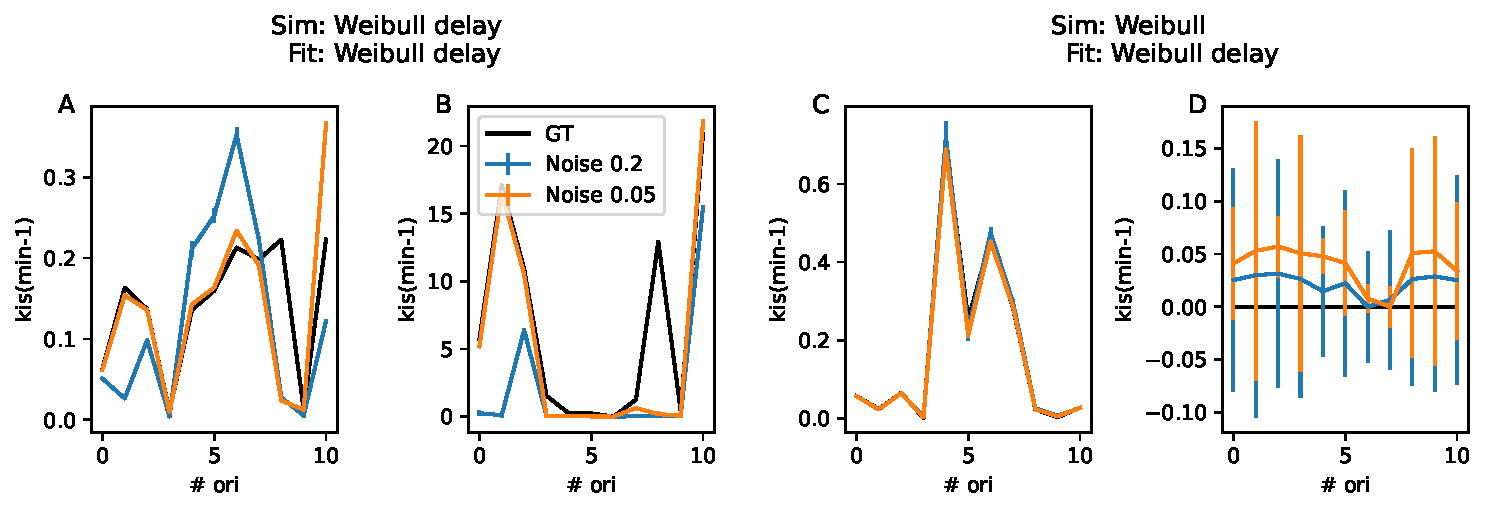
\includegraphics[width=1\textwidth]{figures/Parameter-estimation.pdf}

\caption{Parameter fitting results for Exponential and Weibull simulations under various noise levels. 
Top row: Fit results for Exponential simulations with delay. (A) Fit of origin strength using the Exponential model without delay. (B) Fit of origin strength using the Exponential model with delay. (C) Fit of delay parameters. 
Bottom row: Fit results for Weibull simulations without delay. (D) Fit of origin strength using the Weibull model without delay. (E) Fit of origin strength using the Weibull model with delay. (F) Fit of delay parameters. In each panel, the red, green, and purple curves represent fits for Gaussian noise levels of 0.075, 0.05, and 0.025, respectively. The black line represents the ground truth. The ELBO has been divided by the number of data points fitted.}\label{fig:syntheticparameter}
\end{figure}

Now we investigate if the parameters estimated correspond to the ones used for the simulations.
As the firing type where correctly identified in a noise level corresponding to experiment, we only focused on correct firing type and possible mismatch for selection of delay.
When fitting Weibull simulations with delay using a model with delay (Fig. \ref{fig:syntheticparameter} A), the fit quality improoved, the lower the noise. At the experimental noise level all but one origin strength were correctly identified.
The model confused a strong origin with high delay with a weak origin.
In a similar way, only low noise level allowed correct estimation of time delay.

For Weibull simulations without delay, fitting with a model with delay, provided correct strength and  produced accurate parameter estimates (Fig. \ref{fig:syntheticparameter} D). The model correctly predicted a delay almost null for all origins.

In conclusion, fitting with the correct model yielded strong parameter estimates. Even with mismatched models, reasonable estimates were obtained, especially when fitting with models containing additional parameters.


\subsubsection{Fits of experimental data}


\paragraph{Fit with using detected peaks}

To test our model and gain more insight into the number of origins necessary to reproduce experimental RFD data we used experimental data from \cite{Theulot2022}. As in the synthetic case, we varied the threshold on the peak selection method on the derivative of the RFD, and then computed ELBO and selected the best model.
By doing so we noticed that there could be increase in the ELBO followed by slow decrease and the again a strong increased. This hinted to the fact that the origin selection procedure would select redundant origin. 
We tried two strategies based either on peak heights or prominence of the derivative of the RFD. The former one leads to heigher ELBO, but still with redundant origin. We then randomly pruned origin by selecting them proportionally to $1-E_i$ so that origin with low efficiency would be selected more frequently. 
Above removal, we perform an optimisation and if the ELBO was lower we selected the new configuration to perform 
a new round of pruning. 
We empirically performed a number of pruning rounds equal to the initial number of selected origins.

We illustrate the fit of the data with the best model, 
using the average of the intrinsic strength and delay, 
on the first 7 chromosomes (Fig. \ref{fig:fit_rfd} A). 
When comparing experimental data with simulated ones, 
the Pearson correlation ranged between 0.95 and 0.98 with an average correlation of 0.97. 
The fits for all chromosomes are displayed in Fig \ref{fig:fit_rfd_all}. 
We then compared the MRT obtained from the simulation to rescaled BrdU profiles obtained from nanotiming 
experiment \cite{Theulot2025}. We performed a simple rescaling: the BrdU profile 
were standardised giving sBrdU, then we display $20(1-\text{sBrdU})$. 
We can observe an excellent agreement with this independent experimental dataset. On the unseen data, the pearson correlation ranged
from 0.82 to 0.95 with an average of 0.88. 
Some difference arises for late regions, such as the near telomeres, 
where the experimental profile is flattened. This could be explained by a lower sensitivity from this type of experiment 
in this range temporal range.


\begin{figure}
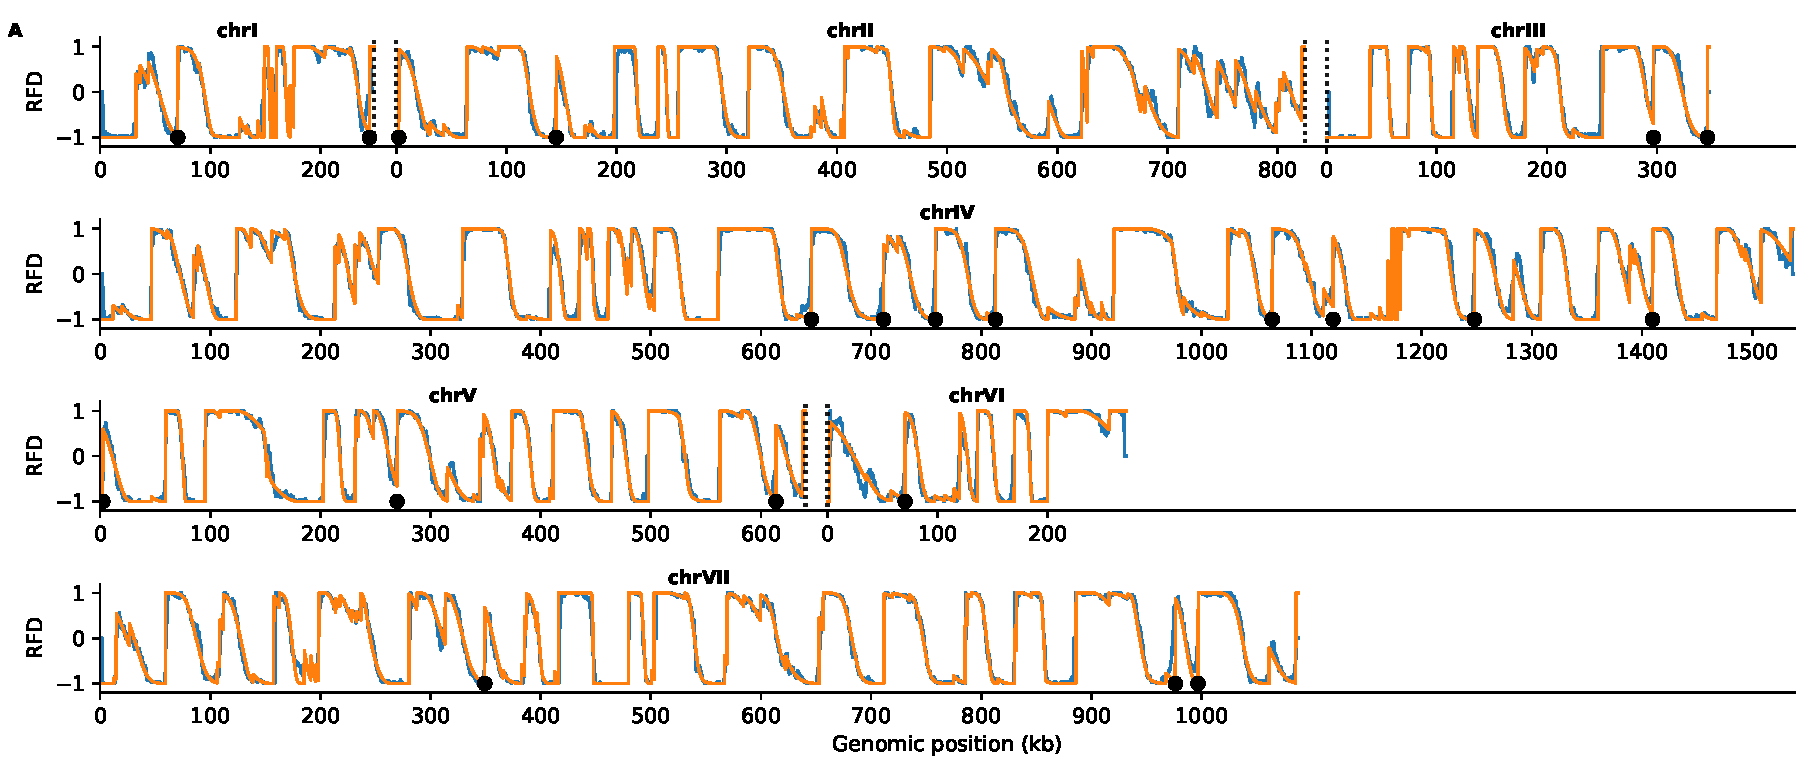
\includegraphics[width=1.0\textwidth]{figures/rfd_compsub.pdf}
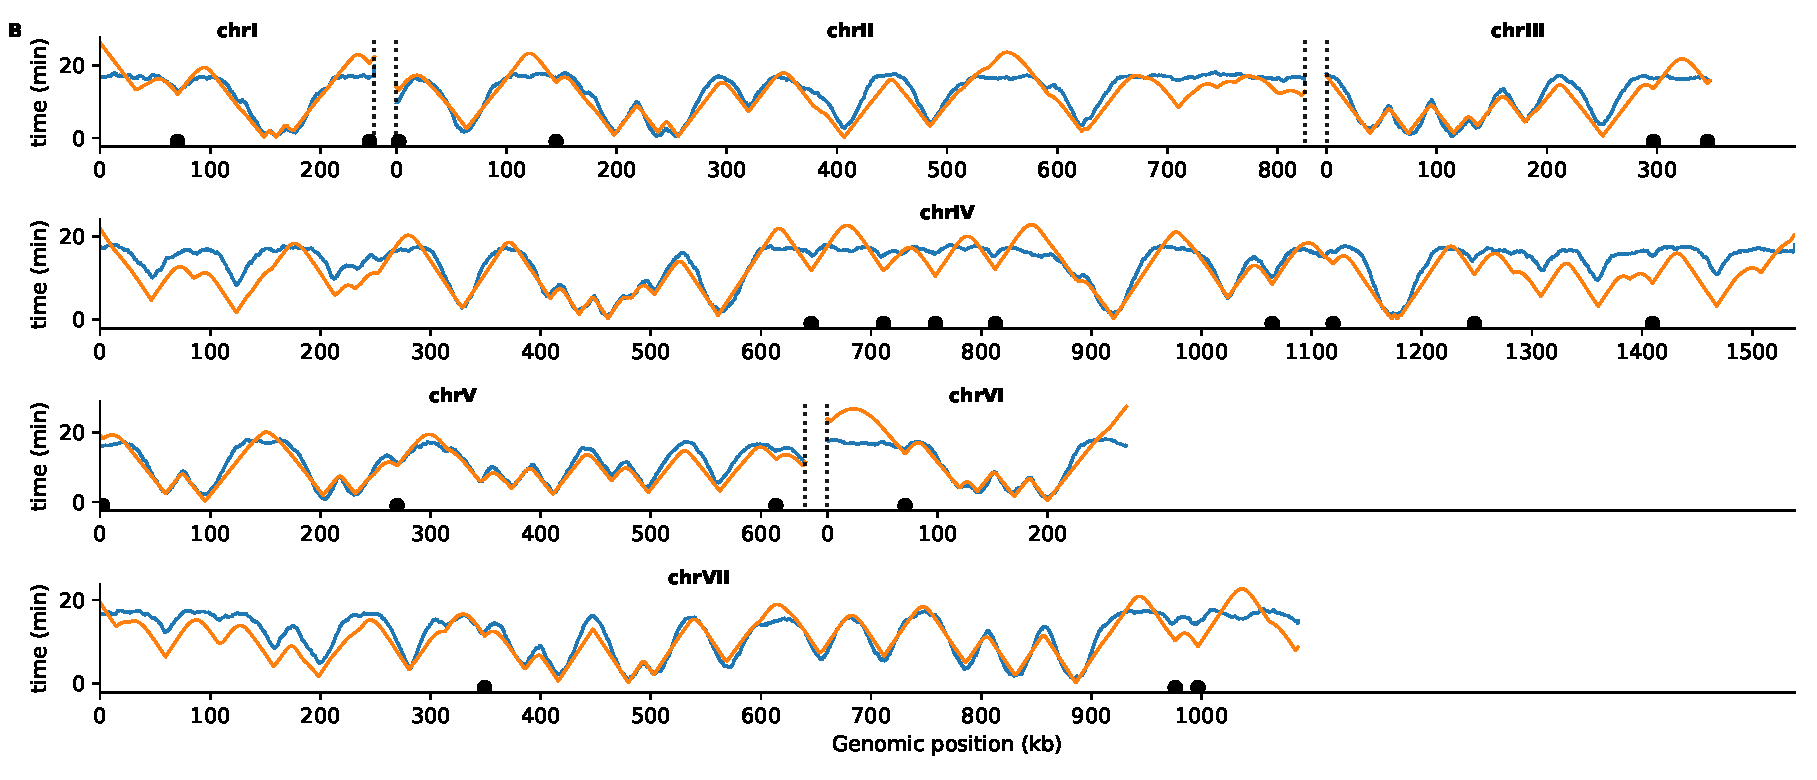
\includegraphics[width=1.0\textwidth]{figures/brdu_repsub.pdf}

\caption{(A) Comparison between experimental (red) and simulated (blue) RFD, for the first 6 chromosomes. The red dot and green dots correspond to origins position. The green are highly delayed origins.  B) Comparison between simulated MRT (red) and rescaled Brdu profile.}\label{fig:fit_rfd}
\end{figure}


When looking at the distribution of origin intrinsic strength and delay (Fig. \ref{fig:fit_elbo} A), we notice that only a small number of origins 45/646 are delayed by more than 1 minute. These highly delayed origins have a rather high observed efficiency (Fig. \ref{fig:fit_elbo} B-C) and have an intermediary replication time (Fig. \ref{fig:fit_elbo} D).
Part of them are located at telomers (eg chrI right telomeres, chrII left telomeres, chrIII right telomers). For those,  we think it could be due to the fact that our simulation do not include capture and release of firing factor. 

\begin{figure}
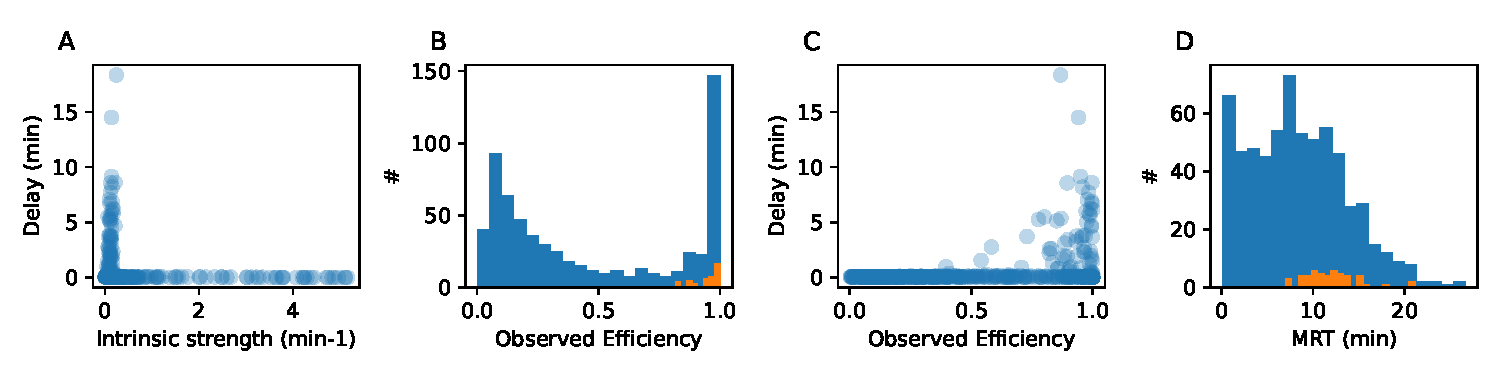
\includegraphics[width=1.0\textwidth]{figures/analyse_ori.pdf}

\caption{A)Scatter plot of Intrinsic strength vs Delay for the 646 origin selected 
B) histogram of the Observed Efficiency for all the orgigns (blue) and for the origin with a delay higher than 1 minute (49 origins) C) Scatter plot of Observed Efficiency vs Delay for all the orgins (blue) and for the origin with a delay higher than 1 minute. D) Histogram of the replication time of all (blue) and high delay origins (orange)}\label{fig:fit_elbo}
\end{figure}

Indeed we tryed fitting our previous model \cite{Arbona2023} that include recycling of firing factor. 
For all the different model the fit where quite good. 
The best model thrgouh ELBO selection was always the Weibull model. 
The only part that where not allmost perfectly fit where located at chromosomes extremities. 
However Fit with delay were better at chromosomes extremities.


\paragraph{Fit with only know origins, Comparison origins / detected peaks}

To add


\section{Discussion}

\paragraph{Model and its Validation}

In this study, we developed analytical models to compute MRT and RFD for genome replication systems with multiple origins, under both exponential and Weibull-distributed firing times. By deriving closed-form expressions for MRT and RFD, we established a computationally efficient Bayesian framework to estimate intrinsic origin efficiencies from experimental data.

Our method achieved high correlations (0.96–0.99) between simulated and experimental RFD profiles across yeast chromosomes (Fig. \ref{fig:fit_rfd}), demonstrating its utility for genome-wide replication timing analyses. Notably, the Weibull model (k=2), which avoids the abrupt firing onset of the exponential distribution, provided marginally better fits to experimental data, as evidenced by higher ELBO values (Fig. \ref{fig:fit_elbo}). This aligns with biological expectations, as origin activation in vivo is unlikely to follow a memoryless process.

Our analysis, through Bayesian model selection, revealed that a model including activation delays provides a better fit for the experimental data. This points to a biologically significant subset of origins whose firing is temporally regulated.

The remarkable correlation between simulated and experimental RFD profiles using inferred intrinsic 
efficiencies demonstrates the model's capacity to capture essential features of the replication landscape. 
This level of accuracy surpasses previous attempts at genome-wide replication modeling in yeast, 
highlighting the power of our analytical approach combined with Bayesian inference. 

The systematic evaluation of model performance across varying origin detection thresholds provides 
robust insights into the replication dynamics of \textit{S. cerevisiae}: our analysis identified 650 
origins as optimal for reproducing experimental Replication Fork Directionality (RFD) profiles, aligning with most studies.

Recent origin mapping in yeast strains revealed ~1,600 potential origins \cite{Foss2024}, but only 500-600 show significant firing under normal conditions \cite{Hennion2020} probably due to the presence of limiting factors required to activate origins \cite{Mantiero2011}. Our model's optimal origin number matches these experimental counts, suggesting the estimated $\lambda_i$ values reflect biological licensing potential filtered through factor availability.

\paragraph{Biological Implications}

Our distinction between $\lambda_i$ (intrinsic firing rate) and $E_i$ (passivation-adjusted probability) provides mechanistic insights. 
While $E_i$ reflects an origin's net contribution to replication, $\lambda_i$ represents its inherent activation potential - 
a critical parameter for studying origin regulation. For example, 
two origins with identical $\lambda_i$ may show different $E_i$ values due to positional effects, as $E_i = \lambda_i \text{MRT}(x_i)$, 
explaining how genomic context modulates replication outcomes.

Future work should focus on elucidating the molecular mechanisms governing these delays, potentially involving chromatin remodeling, 
transcription factor binding, or higher-order chromosome structure.

Our $\lambda_i$ parameter directly corresponds to an origin's ability to recruit limiting initiation factors - a property determined by ACS motif strength and nucleosome positioning \cite{Marks2017,Foss2024}. Chromatin context such as regulation by Rif1 \cite{Peace2014,Theulot2025}, Forkhead transcription factors \cite{Knott2012}, DBf4 at the kinetochore \cite{Natsume2013}, or regulated by trans elements in a larger 3D chromatin context \cite{Knott2012}.

We also identified a subset of origins requiring high delay for activation, whose mechanism should be investigated in future work.

\paragraph{Limitations and Future Directions}

One important hypothesis is that all origins are licensed in each cell. This is not in line with our current knowledge. 
However, we observed that the fits are excellent. We simulated a simple synthetic dataset with the partial licensing at 80\% of 
either a strong origin or a weak origin (Fig. \ref{si:qi}) in the same background. 

From visual inspection, the partial licensing of the weak origin is very similar to having an origin with lower efficiency. 
However, for the strong origin, the signature is quite unique with a plateau around -0.5, a signature that is not visible in our dataset. 
Our  model thus predict that potentially only weak origin are partially licensed, however it is not able to distinguish weak origin always
licensed but rarelly actived from an origin licensed in only a fraction of the cell.
We also proposed a way to integrate mathematically this effect as a perturbation of the full MRT.

While our current framework assumes a constant fork speed, it could be extended to accommodate variable fork speeds. We propose an iterative approach: first, fit the data assuming a constant average speed to obtain an initial MRT profile. Second, use this MRT profile to estimate a position-dependent fork speed. Third, re-calculate the MRT using the variable speed profile. This process could be repeated until the parameter estimates converge, providing a more nuanced picture of replication dynamics.

Another limitation is ignoring the recycling of firing factor that were shown to be critical 
for reproducing the temporal firing rate of origins. 
We investigated this issue by fitting a model incorporating this feature and noticed 
that it affected only subtelomeric regions and that a model with delay was favored. 
However, in the model selection process for the syntetic data, it still favored a model without delay, 
suggesting that the fit of experimental data requiring a delay is not explained by this mechanism.

Another simplification in our approach lies in the variational inference framework, which assumes independence between origin efficiencies (mean-field approximation). While this assumption enables scalable parameter estimation for large systems (e.g., yeast chromosomes with $\sim50-100$ origins), it neglects potential spatial or temporal correlations between neighboring origins. For instance, origins in close proximity may exhibit coordinated licensing or competition for firing factors, phenomena that could bias posterior estimates of their intrinsic efficiencies.

The mean-field approximation also impacts model selection via the ELBO, 
as it underestimates posterior uncertainties. 
In synthetic tests, we observed that the ELBO values allow selection of the correct firing type; 
however, sometimes it did not discriminate between models with or without delay. 
In practice it was not a big issue as the model fitted with delay on data without delay returned a value for the delay close to zero (Fig. \ref{fig:fit_rfd}).

To address these limitations, future work could incorporate structured variational distributions that model pairwise correlations,
 such as multivariate Gaussians with sparse covariance matrices. 
 Spatial priors, such as Gaussian processes with chromosomal-distance-dependent kernels, 
 could further refine efficiency estimates by encoding biophysical constraints (e.g., origin clustering or initiation zone \cite{Petryk2016}). 
 Alternatively, hybrid approaches combining variational inference with Hamiltonian Monte Carlo (HMC) could be employed for small chromosomal regions,
leveraging exact sampling to validate posterior correlations.


\paragraph{Broader Impact}

Our analytical derivations bridge a critical gap between replication theory and data-driven modeling. 
By eliminating the need for stochastic simulations, we enable Bayesian inference on timescales compatible 
with high-throughput sequencing datasets. This opens avenues for studying replication dynamics under varying 
cellular conditions (e.g., stress, cell cycle perturbations) or across species with divergent origin licensing strategies.

In conclusion, while the mean-field assumption represents a pragmatic trade-off for scalability, 
our work establishes a foundation for more sophisticated models of genome replication. 
As single-molecule and sequencing technologies continue to refine spatiotemporal replication maps, 
integrating biophysical correlations into Bayesian frameworks will be essential to unravel the 
complexity of origin regulation in higher eukaryotes.


\bibliography{all_ref.bib} 
\bibliographystyle{ieeetr}
%\printbibliography

\appendix


\section{Deriving MRT from $p_i$}\label{seq:MRT}

\begin{equation}
p_i(x,t) =  p \left(t-\frac{|x-x_i|}{v}\right) 
\end{equation} 

The probability that another fork $j$ arrives at $x$ later than $t$  is given by

\begin{equation}
M_j(x,t) = \int_t^{\infty} p_j(x,\tau) d\tau
\end{equation} 

So the probability that the fork coming from $i$ replicate $x$ at $t$ is

\begin{equation}
P_i(x,t) = p_i(x,t)\prod_{j \neq i} M_j(x,t)
\end{equation}

And the probability for a point $x$ to be replicated at $t$ is 

\begin{equation}\label{op}
P(x,t) = \sum_i P_i(x,t)
\end{equation}

The latter definition forms the base of Retkute al \cite{Retkute2012} model.
Noticing that $p_i(x,t) = -\frac{dM_i}{dt}$ allows to write $P(x,t)$ with a denser form:

\begin{equation}\label{trick}
P(x,t) = -\frac{ d }{dt} \prod_{i} M_i(x,t)
\end{equation}

In fact $s(x,t)=\prod_{i} M_i(x,t)$ is the probability that x has not been replicated at time $t$. This relation-ship as already noted in \cite{Baker2014}. Eq. \eqref{trick} allows us to write a simplified version of the MRT. The MRT is defined by:

\begin{equation}\label{omrt}
MRT(x) =  \int_{0}^{T} t P(x,t) dt
\end{equation}
with $T$ a time that can be taken large with respect to the S-phase but that we will push to infinity at the end of this derivation. Using Eq. \eqref{trick}:

\begin{equation*}
MRT(x) = - \int_{0}^{T} t \frac{ d }{dt} s(x,t) dt
\end{equation*}

and if we integrate by parts and using $s(0,x)=1$ because no DNA as been replicated at time $t=0$.

\begin{equation}\label{mrt0}
MRT(x) =  -T\frac{s(x,T)}{f} + \int_{0}^{T} s(x,t) dt
\end{equation}

As $s(\infty,x)$ tends towards zero faster than $t$ because it is the product of several cumulative distributions, this simplifies Eq. \eqref{mrt0} :



\section{Exponential case}\label{appendix:exponential}

If we consider that the origins follow an exponential law of firing, starting at $t>0$, then
$p_i(t) = H(t)\lambda e^{-\lambda_i t}$
and the cumulative distribution is $F(t) = (1-e^{-H(t)\lambda t})$ with H(t) the Heaviside function.


And so 
\begin{equation}
p_i(t,x) =  H(t-t_i)\lambda_ie^{-H(t-t_i)\lambda_i(t-t_i)}
\end{equation}
and
 
\begin{equation}
M_i(t,x) = 1-F_i \left(t-\frac{|x-x_i|}{v}\right) = e^{-H(t-t_i)\lambda_i(t-t_i)}
\end{equation}
with $t_i =\frac{|x-x_i|}{v} + t_i^S$ the total delay containing two factors. The first one corresponds to the time for the fork to propagate and $t_i^S$ is an optional delay that can be added to mimic a delay in activation of the origin.


To determine $MRT(x)$, we class the $n$ origins by increasing time of arrival to x,  $t_i$. So $t_1 =\frac{|x-x_1|}{v}$ is the closest origin to x. And we cut the integration into pieces: from (0 to $t_1$), all $M_i(t,x)$ are equal to 1. Between $t_1$ and $t_2$ only $M_1(t,x)$ is different from one and:
$s(x,t_1<t<t_2) = e^{-\lambda_1(t-t_1)}$. And more generally:
$s(x,t_i<t<t_{i+1}) = \prod_{j=1}^{i}  e^{-\lambda_j(t-t_j)}$. We also define $t_{n}=\infty$, thus 

\begin{equation}
MRT(x) = t_1+ \sum_{i=1}^{n}\int_{t_i}^{t_{i+1}}e^{-\sum_{j=1}^i \lambda_j(t-t_j)}dt
\end{equation}

\begin{equation}\label{app:mrt_exp}
MRT(x) = t_1 +\sum_{i=1}^{n}\frac{1}{\sum_{j=1}^i \lambda_j}\left[e^{-\sum_{j=1}^i \lambda_j(t_i-t_j)}  -e^{-\sum_{j=1}^i \lambda_j(t_{i+1}-t_j)} \right]
\end{equation}


if we define with $S^i=\sum_{j=1}^i \lambda_j$

then one can show that $MRT^2(x)=- \int_{0}^{T} t^2 \frac{ d }{dt} s(x,t) dt$ is equal to:

\begin{equation}\label{app:mrt_exp2}
MRT^2(x) = t^2_1 +\frac{2}{S^i} \sum_{i=1}^{n} \left[(t_i+1/S^i)e^{-\sum_{j=1}^i \lambda_j(t_i-t_j)}  -(t_{i+1}+1/S^i)e^{-\sum_{j=1}^i \lambda_j(t_{i+1}-t_j)} \right]
\end{equation}
so that the dispersion of the MRT around its mean value is easily computed when computing the MRT.


To derive $E_i$ the observed efficiency, we can notice that given the exponential form of the firing law, $P_i(x,t)=\lambda_i H(t-t_i)s(x,t)$. As $E_i = \int_0^{\infty}P_i(x_i,t)dt$ then

\begin{equation}\label{Ei}
E_i = \int_0^{\infty} \lambda_i H(t-t_i) s(x_i,t)dt = \lambda_i MRT(x_i)
\end{equation}
This is true in the case where there is no delay of activation $t_i^S$ because then $t_i=0$ as the origin is located at position $x_i$.
This relation-ship that link the observed efficiency, the intrinsic strength $\lambda_i$ was derived using several approximations in Arbona et al. \cite{Arbona2023} using a more complex model, and is here a consequence of the exponential firing of the origin.

In the case where $t_i^S \neq 0$, if the index of $t_i$ is k. if k is different from zero, it means that the origin i is activated after forks from origins arrive first at $x_i$ then:

\begin{equation}
E_I = \lambda_I \sum_{i=k}^{n}\frac{1}{\sum_{j=1}^i \lambda_j}\left[e^{-\sum_{j=1}^i \lambda_j(t_i-t_j)}  -e^{-\sum_{j=1}^i \lambda_j(t_{i+1}-t_j)} \right]
\end{equation}



RFD is defined by the derivative of the MRT with respect to $x$: $RFD(x)=v \frac{dMRT(x)}{dx}$. In  Eq. \ref{app:mrt_exp} the dependency as a function of $x$ is implicit in the $t_i$ terms. As  $t_i=|x-x_i|/v$ and $\frac{dt_i}{dx}=\sign(x-x_i)/v=d_i/v$ with d stating for direction


\begin{equation}
RFD(x) = d_1 + \sum_{i=1}^{n}\frac{1}{\sum_{j=1}^i \lambda_j}(A_{i,i+1}-A_{i,i})
\end{equation}

with
\begin{equation}
A_{i,k} =e^{-\sum_{j=1}^i \lambda_j(t_k-t_j)} \sum_{j=1}^i \lambda_j(d_k-d_j)
\end{equation}


\section{Analytical formulas Weibull distribution with $k=2$}\label{appendix:weibull}


For the Weibull distribution with $k=2$, the probability for an origin to fire is $p(t) =  H(t)2t\lambda_i^2e^{-(\lambda_i t)^2}$
and the cumulative distribution is $F(t)=1-e^{-H(t)(\lambda_i  t)^2}$.

By sorting again the origin by time of arrival:
\begin{equation}
MRT(x) = t_1+ \sum_{i=1}^{n}\int_{t_i}^{t_{i+1}}e^{-\sum_{j=1}^i (\lambda_j(t-t_j))^2}dt
\end{equation}

and by completing the square of the Gaussian integral one get
\begin{equation}
MRT(x) = t_1 + \sum_{i=1}^{n}MRT_i(x)
\end{equation}

with 

\begin{equation}
MRT_i(x)=\frac{1}{\sqrt{\avgk 1}}e^{\avgk t ^2/\avgk 1-\avgk {t^2}}\int_{\sqrt{\avgk 1}(t_i-\avgk t /\avgk 1)}^{\sqrt{\avgk 1}(t_{i+1}-\avgk t /\avgk 1)}e^{-u^2}du
\end{equation}


with $\avgk a = \sum_{j=1}^{i}\lambda_j^2 a_j$ for any list $a=(a_1,a_2,...,a_N)$ and $\avgk 1= \sum_{j=1}^{i}\lambda_j^2$. The integral part of $MRT_i(x)$ is the Gauss error function between two times which can be computed quickly as good analytical analytical approximation are known. 

For the second moment:

\begin{equation}\label{app:mrt_wei}
MRT^2(x) = t^2_1  + \sum_{i=1}^{n} \left(\frac{2\avgk t MRT_i(x)}{\avgk 1}  - \frac{1}{\avgk 1} \left[ e^{-\sum_{j=1}^i (\lambda_j(t-t_j))^2}\right]_{t_i}^{t_{i+1}} \right)
\end{equation}

For the Observed efficiency unfortunately the relation-ship with $MRT(x)$ is not as simple as in the exponential case. First the $MRT_i(x)$ term can be decomposed in $MRT_i(x)=F_i I_i$ with 
\begin{equation}
F_i=\frac{1}{\sqrt{\avgk 1}}e^{\avgk t ^2/\avgk 1-\avgk {t^2}}
\end{equation}
and 


\begin{equation}
I_i=\int_{\sqrt{\avgk 1}(t_i-\avgk t /\avgk 1)}^{\sqrt{\avgk 1}(t_{i+1}-\avgk t /\avgk 1)}e^{-u^2}du
\end{equation}

So that the efficiency of origin $l$ is:

\begin{equation}
E_l =  2\lambda_l \sum_{i=k}^{n}\int_{t_i}^{t_{i+1}}(t-t_l)e^{-\sum_{j=1}^i (\lambda_j(t-t_j))^2}dt
\end{equation}
where the sum starts at  $k$, the index of $t_l$, as in the exponential case. 

\begin{equation}
E_l = 2\lambda_l^2\sum_{i=k}^{n} F_i\left[\left(\frac{\avgk t}{\avgk 1}-t_l\right)I_i
 +\frac{1}{2 \sqrt{\avgk 1}} \left[ e^{-\avgk 1\left(t_i-\frac{\avgk t}{\avgk 1}\right)^2} - e^{-\avgk 1\left(t_{i+1}-\frac{\avgk t}{\avgk 1}\right)^2}\right]\right]
\end{equation}

For the RFD,

\begin{equation}
RFD(x) = d_1+ \sum_{i=1}^{n}RFD_i(x)
\end{equation}
with

\begin{equation}
RFD_i(x) = F_i\left(2 I_i \left(\frac{\avgk t}{\avgk 1} \avgk d - \avgk {td}\right) + \delta I_{i,i+1}-\delta I_{i,i}\right)
\end{equation}

with 
\begin{equation}
\delta I_{i,k} = \sqrt{\avgk 1}\left(s_{k}-\frac{\avgk s}{\avgk 1}\right)e^{-\avgk 1 \left(t_{k}-\frac{\avgk t}{\avgk 1}\right)^2}
\end{equation}

\section{RFD jump}\label{seq:rfdj}

For a two origins system:
\begin{equation}
RFD(x) = d_1 + \frac{1}{\lambda_1}(A_{1,2}-A_{1,1})+\frac{1}{\lambda_1+\lambda_2}(A_{2,3}-A_{2,2})
\end{equation}
$A_{1,1}=0$ as well as $A_{3,2}$.

Then 
\begin{equation}
RFD(x) = d_1 + \frac{1}{\lambda_1}(\lambda_1(d_2-d_1)e^{-\lambda_1(t_2-t_1)})+\frac{1}{\lambda_1+\lambda_2}(-\lambda_1(d_2-d_1)e^{-\lambda_1(t_2-t_1)})
\end{equation}
as $t_1\approx 0$ around $x=x_1$
one get 

\begin{equation}
RFD(x) = d_1 + (d_2-d_1)e^{-\lambda_1 t_2}-\frac{\lambda_1}{\lambda_1+\lambda_2}(d_2-d_1)e^{-\lambda_1 t_2}
\end{equation}

So the RFD jump is

\begin{equation}
RFD(x_1+\delta)-RFD(x_1-\delta) \approx 2\left(1 - e^{-\lambda_1 t_2}(1-\frac{\lambda_1}{\lambda_1+\lambda_2})\right)  \approx 2E_1
\end{equation}

\section{Detail of parameters prior and likelihood for the RFD:}\label{sup:detail}

In practice we perform 10 optimisations with random seed and select the optimisation result with higher ELBO.
Priors to the parameters $\lambda_i$ were chosen as Weibull (k=2) efficiencies (mean $= T_s/2$) and exponential-distributed activation delays with mean $= T_s/5$ for models with delay. 
Typically RFD residuals were modeled as $\mathcal{N}(0,\sigma)$. Also we noticed that stabler result where obtained when fitting not the RFD but $\int_x^{x+1.5\text{kb}}\text{RFD}(u)du = v (\text{MRT}(x+1.5\text{kb})-\text{MRT}(x))$.
As a consequence on synthetic data, where we simulated data at a 100~bp resolution and then added some gaussian noise $\mathcal{N}(0,\text{noise})$ the error $\sigma$ was estimated as $noise/nbins^{0.5}$, where noise is the value of the introduced noise and $nbins$ represents the number of bins in 1.5 kb. This is because for this simulated data, the noise at each bin is uncorrelated. For experimental data, the error for each bin was estimated as $p(x)(1-p(x))/(n(x)+20)$, where $p(x)=(RFD(x)+1)/2$ and $n(x)$ the number of fork in bin $x$ (20 was added to the fork number to prevent overestimation of the confidence interval). This quantity $p(x)$ can be seen as the probability for a fork to go to the right. However, contrary to the simulated data we used $sigma =  p(x)(1-p(x))/(n(x)+20)$ without dividing by the square of the number of bins, as the data coming from single cell molecule is highly correlated on the 1.5 kb scale.

\section{Origin Detection Algorithm}\label{app:origin_detect}

Origin positions were identified through peak detection on the replication fork directionality (RFD) derivative. The pipeline comprises three steps:

\begin{enumerate}
    \item \textbf{Smoothing}: RFD profiles were convolved with a Gaussian kernel ($\sigma=3$ kb) to reduce high-frequency noise:
    \begin{equation}
        \text{RFD}_{\text{smooth}}(x) = \text{RFD}(x) \ast \frac{1}{\sigma\sqrt{2\pi}}e^{-\frac{x^2}{2\sigma^2}}
    \end{equation}
    
    \item \textbf{Differentiation}: The numerical derivative was computed using central differences:
    \begin{equation}
        \frac{d\text{RFD}}{dx} \approx \frac{\text{RFD}(x+\Delta x) - \text{RFD}(x-\Delta x)}{2\Delta x}, \quad \Delta x = 100\ \text{bp}
    \end{equation}
    
    \item \textbf{Peak Detection}: Local maxima in $|d\text{RFD}/dx|$ were identified using SciPy's \texttt{find\_peaks} with:
    \begin{itemize}
        \item Minimum prominence: $0.001$ per 100 bp
        \item Minimum inter-peak distance: 3 kb
        \item Height threshold: $>5\times$ median absolute deviation
    \end{itemize}
\end{enumerate}


\section{Fit all:}

\begin{figure}
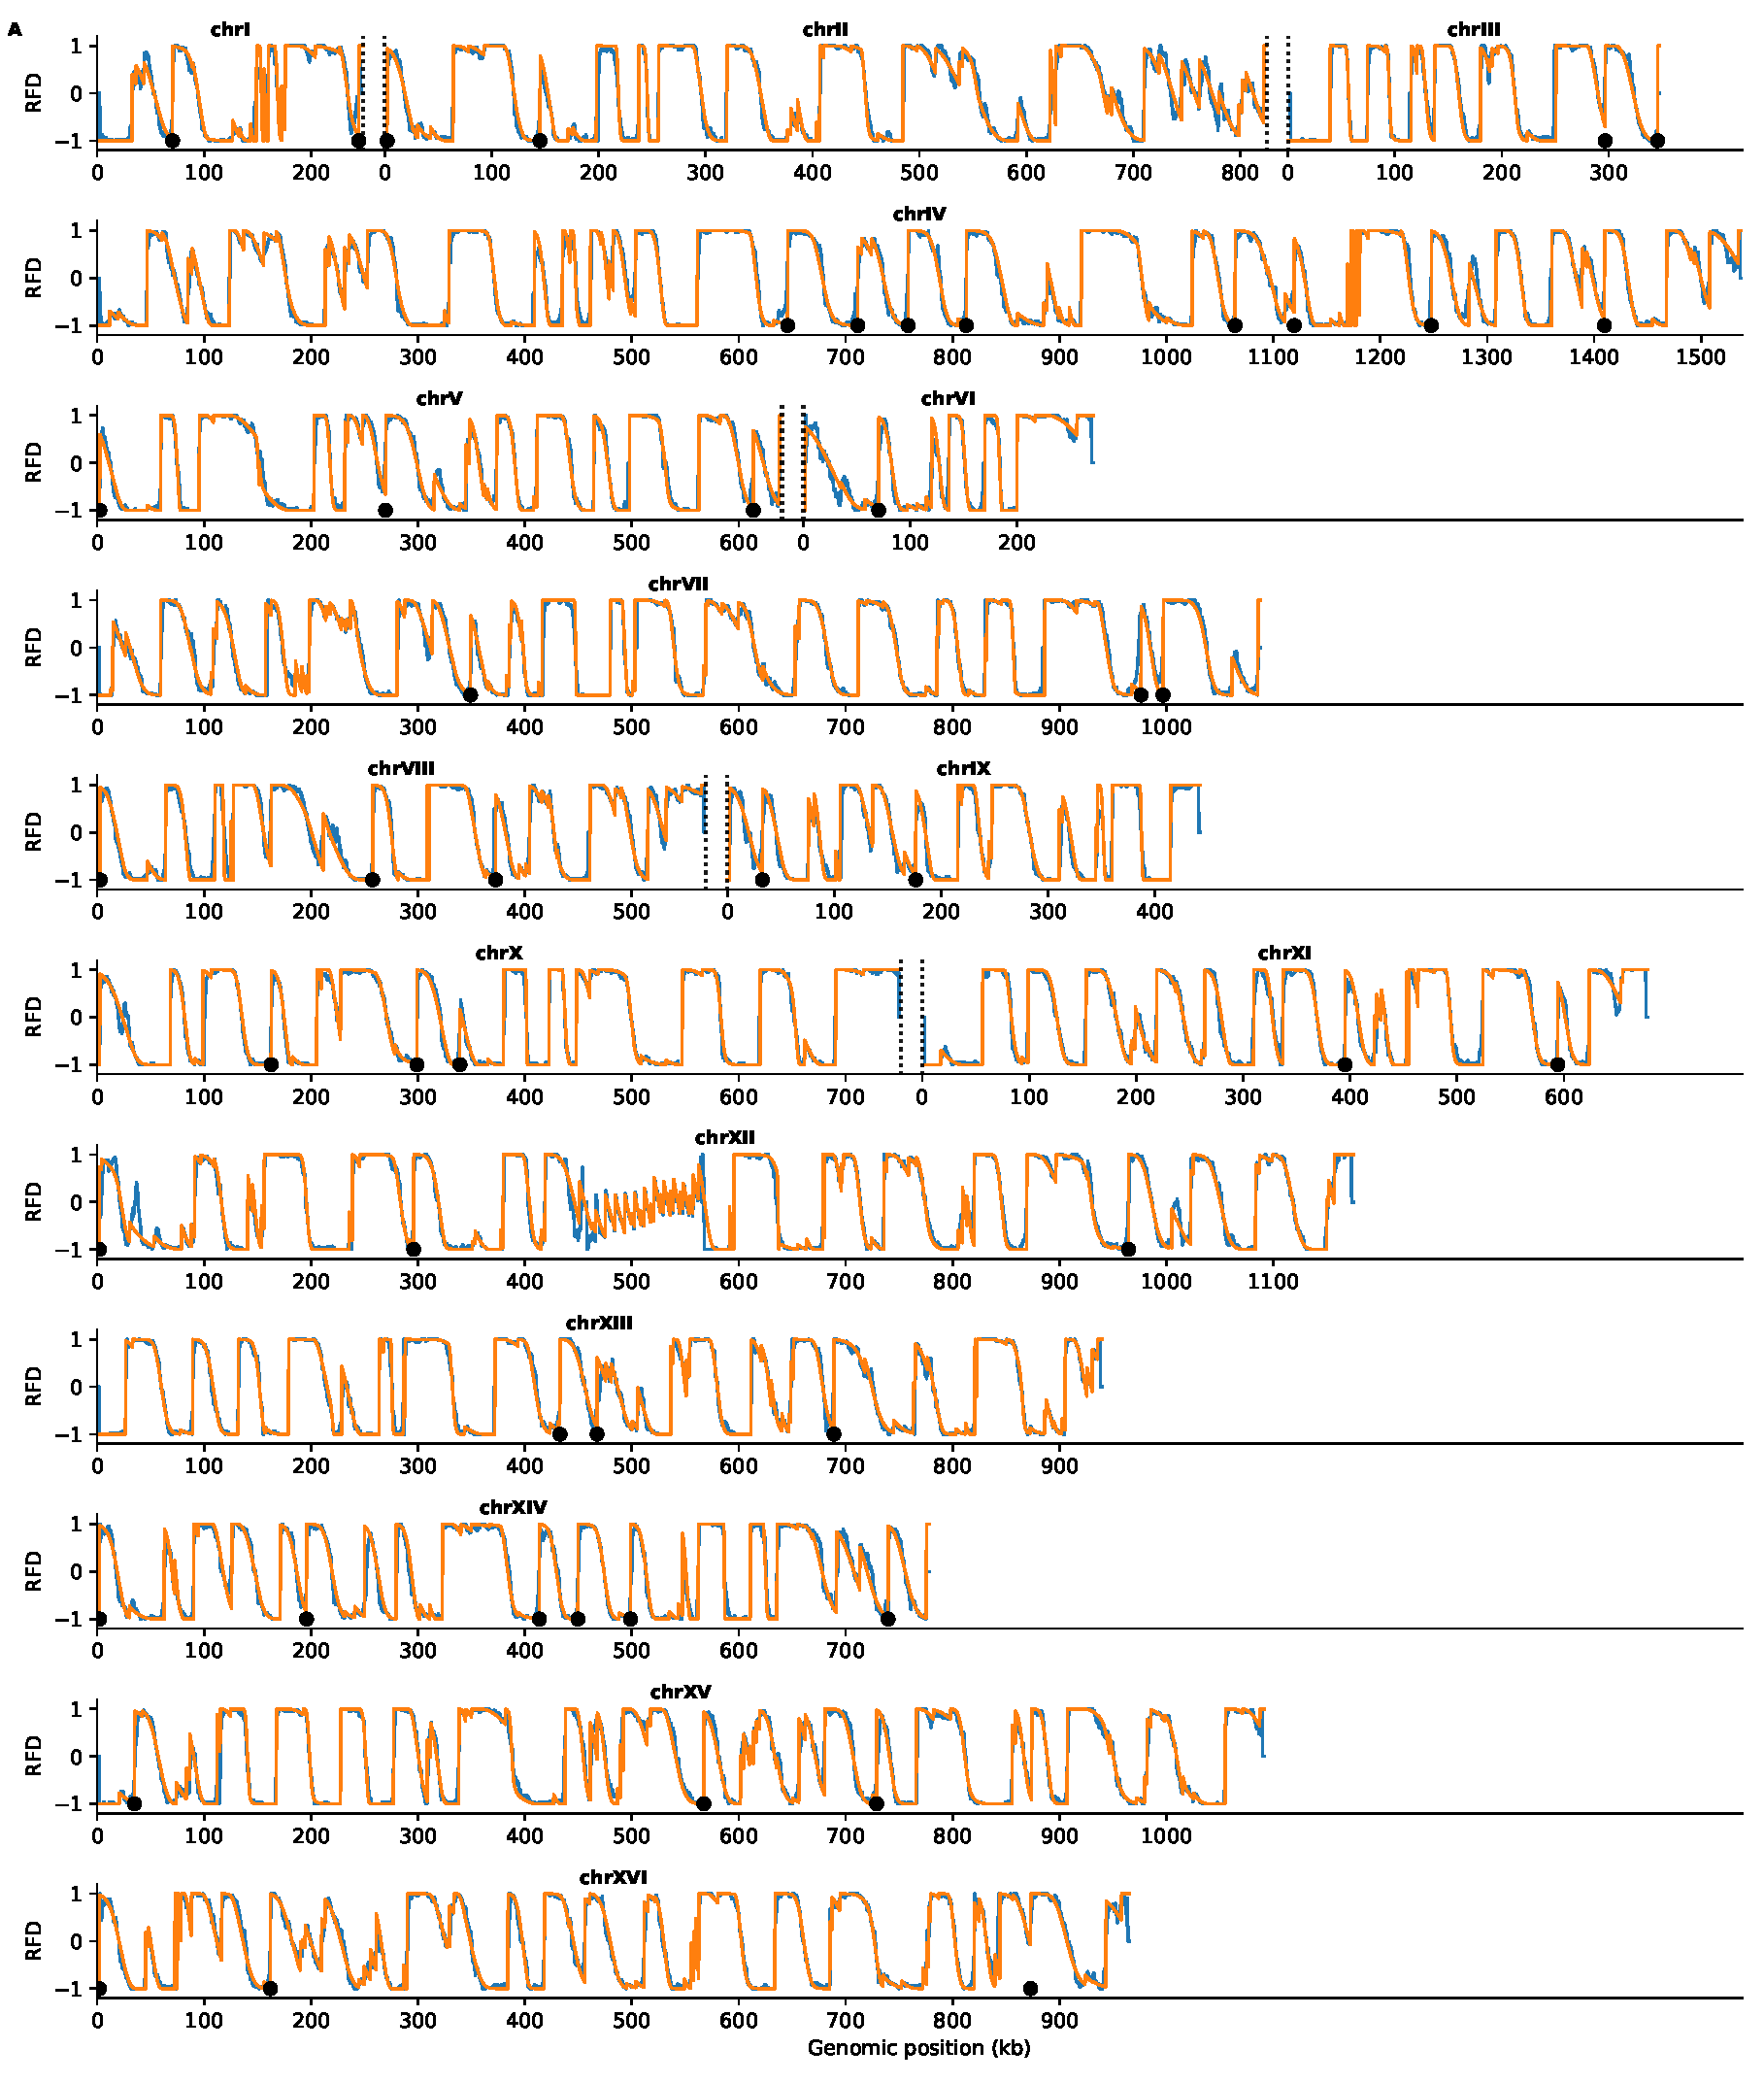
\includegraphics[width=1.0\textwidth]{/home/jarbona/reports/Article-MathMod/figures/rfd_compfull.pdf}

\caption{(A) Comparison between experimental (red) and simulated (blue) RFD, for all the chromosomes. The red dot indicates the positioning of the origins, the green corresponds to origins with high delay.}\label{fig:fit_rfd_all}
\end{figure}


\begin{figure}
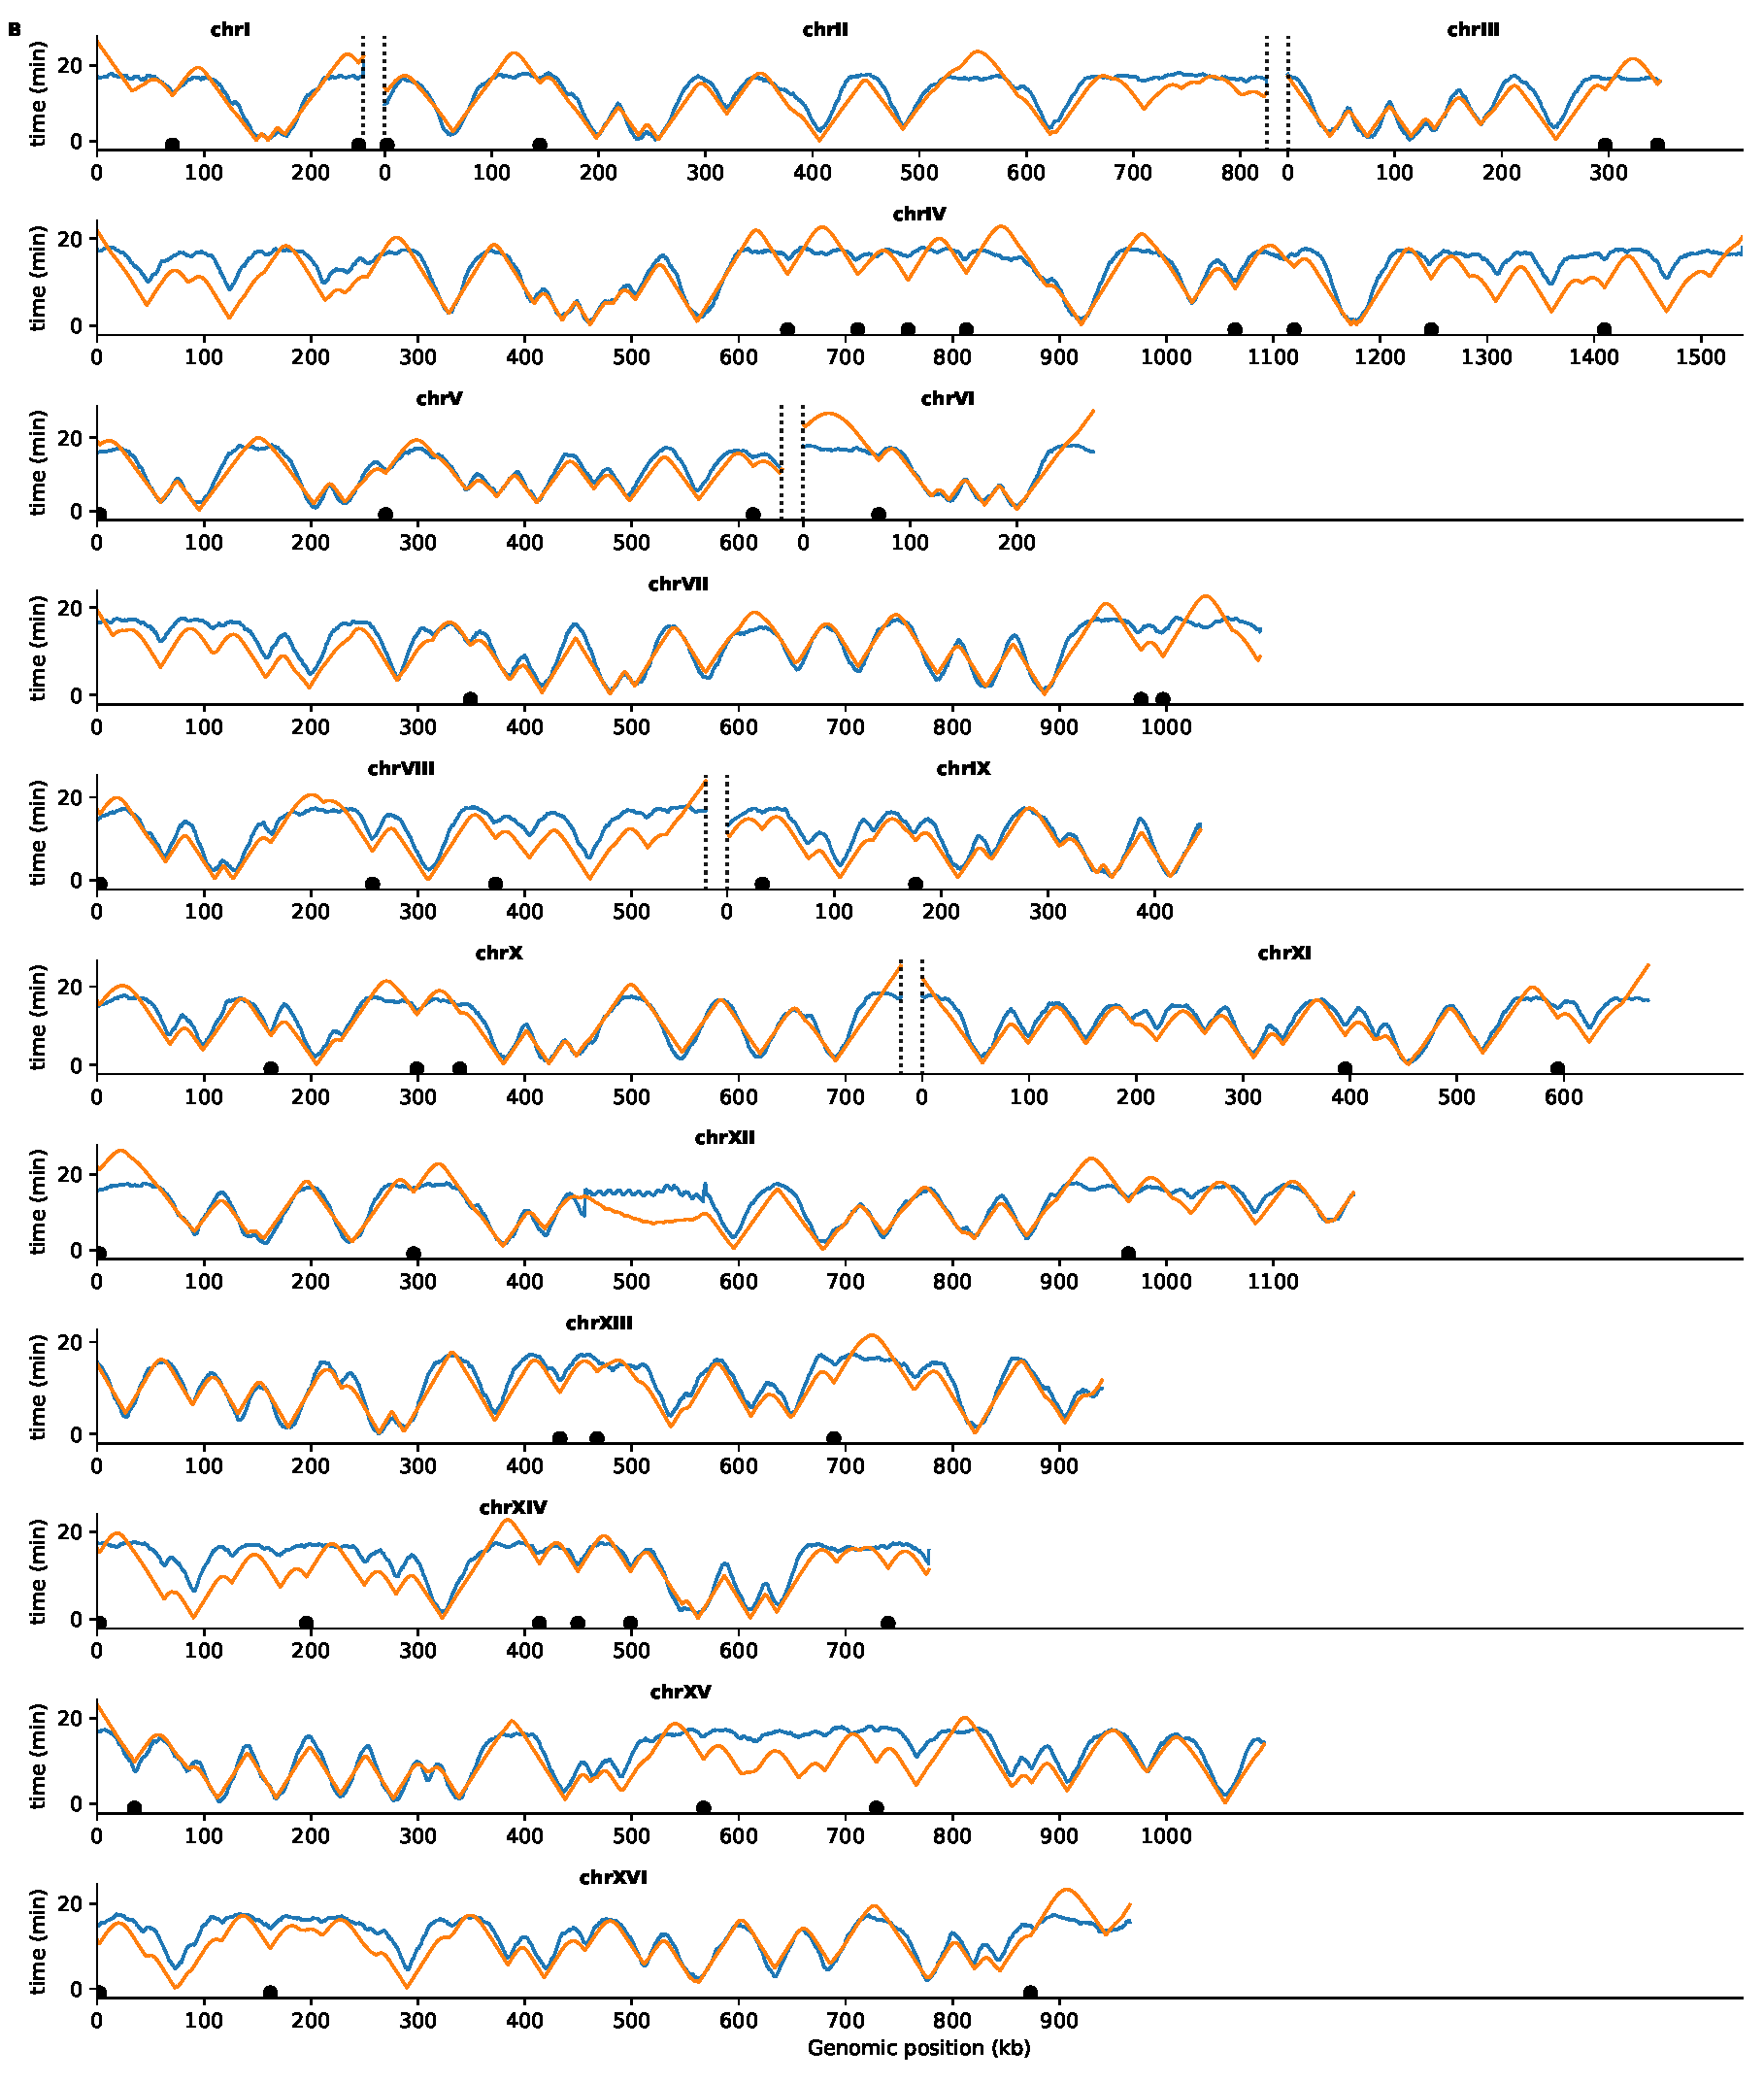
\includegraphics[width=1.0\textwidth]{/home/jarbona/reports/Article-MathMod/figures/brdu_repfull.pdf}

\caption{(A) Comparison between experimental (red) and simulated (blue) RFD, for all the chromosomes. The red dot indicates the positioning of the origins, the green corresponds to origins with high delay.}\label{fig:fit_rfd_all_brdu}
\end{figure}


\begin{figure}
\includegraphics[width=1.0\textwidth]{/home/jarbona/reports/Article-MathMod/figures-old//fitting-qidiscussion.pdf}

\caption{Comparison of a system with full licensing (blue) , partial licensing of the second origin (weak), or partial licensing of the fourth origin (strong) for MRT (left) and RFD (right) }\label{si:qi}
\end{figure}


%\section{Alternative-data}
%
%\begin{figure}
%\includegraphics[width=1.0\textwidth]{/home/jarbona/reports/Article-MathMod/figures/fitted_RFD-WT.pdf}
%\includegraphics[width=1.0\textwidth]{/home/jarbona/reports/Article-MathMod/figures/fitted_RFD.pdf}
%
%\caption{(A/B) Comparison between experimental (red) and simulated (blue) RFD, for the first 6 chromosomes. The red dot indicates the positioning of the origins, the green corresponds to origins with high delay. A correspond to WT, while B the TOF1 mutant.}\label{fig:fit_rfd2}
%\end{figure}
%
%To gain more insight into the number of origin necessary to reproduce the RFD data, as in the synthetic case, we varied the threshold on the peak selection method on the derivative of the RFD,
%and then computed ELBO and selected the best model.
%We illustrate the fit of the data with the best model,using the average of the intrinsic strength and delay, on the first 6 chromosome for a WT strain Fig. \ref{fig:fit_rfd} A) and for a TOF1 mutant strain  Fig. \ref{fig:fit_rfd} B).
%
%When comparing experimental data with simulated ones, the pearson correlation ranged between 0.97 and 0.99 with an average correlation of 0.98, for the WT strain, and a sligthly lower correlation for the TOF1 strain, with a mean of 0.97 and a range between 0.96-0.98.
%
%
%\begin{figure}
%\includegraphics[width=1.0\textwidth]{/home/jarbona/reports/Article-MathMod/figures/ELBO-WT.pdf}
%\includegraphics[width=1.0\textwidth]{/home/jarbona/reports/Article-MathMod/figures/ELBO.pdf}
%
%\caption{A/E) Sum of ELBO for each chromosomes, divided by the total number of RFD points, as a function of the number of origins in the Weibull and Exponential case with and without time shift B/F) Scatter plot of average origin intrinsic strength against the average stimated time delay, C/G) Histogram of observed efficiency for all (blue) or only origin with high delay (superior to 1 min, orange) . D/H) Histogram of the replicaton time of all (blue) and high delay origins (orange). The first line correspond to WT strain and the second one to TOF1.}\label{fig:fit_elbo2}
%\end{figure}
%
%
%
%
%In Fig. \ref{fig:fit_elbo} A/E we report the sum of the ELBO for each chromosomes for each model for the wild type strain (A) and the TOF1 mutant (E). As in the synthetic case for very low number of origin the ELBO is very low, and then a maximum appears. In both cases, the Weibull models have higher ELBO that the Exponential one, the best model being the Weibull model with time delay. However in the WT strain the difference between the Weibull and Exponential models with delay is small. For the WT strain ll the different models estimate consistently the number of origin necessary to reproduce the data between 850 and 900 wild in the TOF1 mutant it is betmeen 500-600. For the best model the estimated number of origin are of 956 and 599. When looking at the distribution of origin intrinsic strength and delay (Fig. \ref{fig:fit_elbo} B), we notice that only a small number of origin 185/956 and 58/599 have had a delay over 1 minutes. These high delay origin have rather high observed efficiency (Fig. \ref{fig:fit_elbo} C/G) and have an intermediary replication time ( (Fig. \ref{fig:fit_elbo} D/H). The number of origin requiered to fit the data are rather different between the two strains. This difference can be explained by a difference of coverage the WT strain has an average coverage of 440 while the TOF1 mutant has an average coverage of 30. Thus the procedure accounts correctly for the error an fit finer detail for the WT. However, judging by the eye (Fig. \ref{fig:fit_rfd} A), it seems that the model sligthly over fit, especially if flat high plateau were it estimates that it needs several origin to fit. This can be observed also by a large population of low efficiency origins present in (Fig. \ref{fig:fit_elbo} C) but not in (Fig. \ref{fig:fit_elbo} G).



\end{document}
